\documentclass{article}

\usepackage[preprint]{neurips_2025}

%=============================================================================
% PACKAGES
%=============================================================================
\usepackage[utf8]{inputenc}
\usepackage[T1]{fontenc}
\usepackage{hyperref}
\usepackage{url}
\usepackage{booktabs}
\usepackage{amsfonts}
\usepackage{amssymb}
\usepackage{amsmath}
\usepackage{nicefrac}
\usepackage{microtype}
\usepackage{xcolor}
\usepackage{graphicx}
\usepackage{multirow}
\usepackage{colortbl}
\usepackage{enumitem}
\usepackage{siunitx}

% TikZ for diagrams
\usepackage{tikz}
\usetikzlibrary{positioning, arrows.meta, shapes.geometric, fit, backgrounds}

% Graphics path
\graphicspath{{figures/}}

%=============================================================================
% METADATA
%=============================================================================
\title{Evaluating Spatial Reasoning in Vision-Language Models: \\
A Diagnostic Benchmark with Mechanistic Analysis}

\author{%
  Lauren Hyoseo Yoon\thanks{Equal contribution. Listing is alphabetical.} \\
  Computation and Neural Systems \\
  California Institute of Technology \\
  \texttt{laurenhyoon@caltech.edu}
  \And
  Xue Ru Zhou$^*$ \\
  Electrical Engineering \\
  California Institute of Technology \\
  \texttt{xzhou5@caltech.edu}
}

%=============================================================================
% DOCUMENT
%=============================================================================
\begin{document}

\maketitle

%-----------------------------------------------------------------------------
% ABSTRACT
%-----------------------------------------------------------------------------
\begin{abstract}
We present a systematic benchmark for evaluating spatial reasoning in vision-language models (VLMs), decomposing spatial understanding into interpretable dimensions: egocentric versus allocentric perspective-taking, viewer-centered versus object-relative reference frames, and multiple spatial relation axes. Our benchmark employs automated ground truth generation from scene images using segmentation and depth estimation, enabling exact-match evaluation across \num{3672} queries. Evaluating three state-of-the-art VLMs, we find consistent performance gaps between egocentric and allocentric reasoning (11--25 percentage points), with allocentric tasks requiring perspective transformation proving substantially harder. Through mechanistic analysis of internal activations and attention patterns, we identify distinct failure mechanisms: egocentric failures correlate with insufficient visual attention (grounding failures), while allocentric failures show no attention deficit (reasoning failures). These findings suggest that improving spatial reasoning requires task-specific interventions rather than uniform approaches.
\end{abstract}

%-----------------------------------------------------------------------------
% INTRODUCTION
%-----------------------------------------------------------------------------
\section{Introduction}
\label{sec:intro}

% TODO: Write introduction
% - Motivation: spatial reasoning is fundamental for embodied AI
% - Problem: existing benchmarks conflate detection, localization, and reasoning
% - Solution: our diagnostic benchmark isolates spatial reasoning
% - Contributions: benchmark + evaluation + mechanistic analysis

%-----------------------------------------------------------------------------
% BACKGROUND / RELATED WORK
%-----------------------------------------------------------------------------
\section{Related Work}
\label{sec:related}

%=============================================================================
% RELATED WORK SECTION
%=============================================================================

\paragraph{Spatial reasoning benchmarks.}
Evaluating spatial understanding in vision-language models has attracted considerable attention, yet existing benchmarks often conflate distinct cognitive abilities. The Visual Spatial Reasoning (VSR) dataset \cite{liu2023vsr} tests binary spatial relations between objects but relies on natural images where object recognition difficulty varies across samples. \citet{kamath2023whatsup} systematically probe VLMs on basic spatial relations and find consistent failures on vertical and horizontal judgments, though their evaluation focuses on absolute positions rather than relational reasoning. SpatialVLM \cite{chen2024spatialvlm} introduces metric distance estimation but does not decompose spatial reasoning into interpretable dimensions. Our benchmark addresses these limitations by isolating spatial reasoning from perceptual confounds through labeled visualizations, decomposing queries along egocentric-allocentric and viewer-object axes, and providing geometrically-computed ground truth that enables exact-match evaluation without annotation ambiguity.

\paragraph{Spatial cognition in vision-language models.}
Large vision-language models have demonstrated impressive capabilities across diverse tasks, yet their spatial reasoning abilities remain poorly characterized. GPT-4V \cite{openai2024gpt4} and Claude \cite{anthropic2024claude} exhibit emergent spatial understanding but lack systematic evaluation across spatial reasoning dimensions. Open-source models like Qwen2-VL \cite{wang2024qwen2vl} and LLaVA \cite{liu2024llava} have closed the gap on many vision-language tasks but show variable performance on spatial queries. Cognitive science distinguishes egocentric representations (viewer-centered) from allocentric representations (object-centered or world-centered) \cite{klatzky1998allocentric, burgess2006spatial}, with allocentric reasoning requiring mental transformation analogous to the classic mental rotation paradigm \cite{shepard1971mental}. Our benchmark operationalizes this distinction, enabling direct measurement of how well VLMs perform perspective transformation---a capability essential for embodied AI applications \cite{driess2023palme, brohan2023rt2} where agents must reason about spatial relations from viewpoints other than their own.

\paragraph{Mechanistic interpretability of visual reasoning.}
Understanding how neural networks implement reasoning has progressed substantially through mechanistic interpretability research. Work on transformer circuits \cite{elhage2021mathematical, olsson2022context} has revealed interpretable computational structures in language models, while recent scaling of these techniques to frontier models \cite{templeton2024scaling} demonstrates that meaningful features can be extracted from large-scale systems. For vision-language models, \citet{gandelsman2024interpreting} decompose CLIP representations via text-based analysis, revealing how visual concepts are encoded. However, mechanistic analysis of spatial reasoning in VLMs remains largely unexplored. Our work contributes to this direction by analyzing internal activations and attention patterns during spatial queries, identifying distinct failure mechanisms for egocentric versus allocentric tasks. This diagnostic approach moves beyond aggregate accuracy metrics to characterize how spatial reasoning succeeds or fails at the computational level.


%-----------------------------------------------------------------------------
% METHODOLOGY
%-----------------------------------------------------------------------------
%=============================================================================
% METHODOLOGY SECTION
% For inclusion in main NeurIPS 2025 document
%=============================================================================
%
% USAGE: Replace your Pipeline section with %=============================================================================
% METHODOLOGY SECTION
% For inclusion in main NeurIPS 2025 document
%=============================================================================
%
% USAGE: Replace your Pipeline section with %=============================================================================
% METHODOLOGY SECTION
% For inclusion in main NeurIPS 2025 document
%=============================================================================
%
% USAGE: Replace your Pipeline section with \input{methodology_section}
%
% REQUIRED PACKAGES - Add to your main.tex preamble:
%   \usepackage{tikz}
%   \usetikzlibrary{positioning, arrows.meta, shapes.geometric, fit, backgrounds}
%
%=============================================================================

\section{Methodology}
\label{sec:methodology}

We present a benchmark for evaluating spatial reasoning in vision-language models that isolates relational reasoning from perceptual confounds. By providing labeled scene visualizations and structured queries with geometrically-computed ground truth, we enable precise diagnosis of model capabilities across spatial reasoning dimensions. Figure~\ref{fig:pipeline} illustrates our two-stage pipeline.

\begin{figure}[t]
\centering
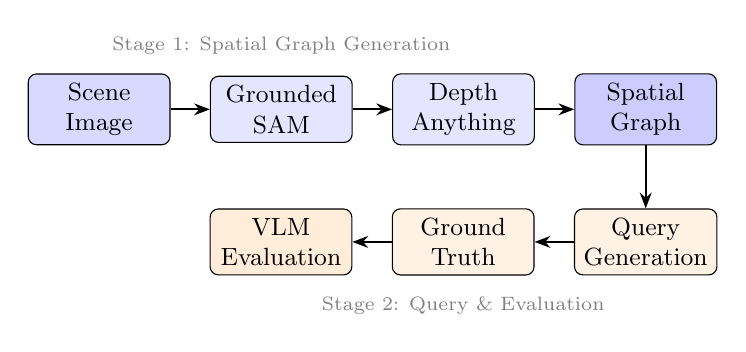
\begin{tikzpicture}[
    node distance=0.4cm,
    box/.style={rectangle, draw, rounded corners=3pt, minimum width=1.8cm, minimum height=0.6cm, align=center, font=\small},
    arrow/.style={-{Stealth[length=2mm]}, thick},
    label/.style={font=\scriptsize, color=gray}
]
% Stage 1: Spatial Graph Generation
\node[box, fill=blue!15] (img) {Scene\\Image};
\node[box, fill=blue!10, right=0.5cm of img] (det) {Grounded\\SAM};
\node[box, fill=blue!10, right=0.5cm of det] (depth) {Depth\\Anything};
\node[box, fill=blue!20, right=0.5cm of depth] (graph) {Spatial\\Graph};

% Stage 2: Query Generation & Evaluation
\node[box, fill=orange!10, below=0.8cm of graph] (query) {Query\\Generation};
\node[box, fill=orange!10, left=0.5cm of query] (gt) {Ground\\Truth};
\node[box, fill=orange!15, left=0.5cm of gt] (eval) {VLM\\Evaluation};

% Arrows
\draw[arrow] (img) -- (det);
\draw[arrow] (det) -- (depth);
\draw[arrow] (depth) -- (graph);
\draw[arrow] (graph) -- (query);
\draw[arrow] (query) -- (gt);
\draw[arrow] (gt) -- (eval);

% Stage labels
\node[label, above=0.15cm of det] {Stage 1: Spatial Graph Generation};
\node[label, below=0.15cm of gt] {Stage 2: Query \& Evaluation};

\end{tikzpicture}
\caption{Pipeline overview. Stage 1 constructs a spatial graph encoding object locations and relations. Stage 2 generates queries with geometric ground truth for exact-match evaluation.}
\label{fig:pipeline}
\end{figure}

\subsection{Spatial Graph Generation}

Given an input image, we construct a spatial graph $G = (V, E)$ where nodes $V$ represent detected objects and edges $E$ encode pairwise spatial relations. Each node stores object metadata (label, bounding box, segmentation mask, depth), and each edge stores the spatial relation between the connected objects.

\paragraph{Object detection and segmentation.} We employ Grounded-SAM, combining Grounding DINO for open-vocabulary detection with SAM for precise mask generation. Given a set of object category prompts, the model returns bounding boxes and segmentation masks for all detected instances. Each object receives a unique identifier by appending an instance index to its category label (e.g., \texttt{chair\_0}, \texttt{chair\_1}). We filter detections by confidence threshold and remove heavily overlapping boxes via non-maximum suppression.

\paragraph{Depth estimation.} We apply Depth Anything V2 to obtain a dense relative depth map $D \in \mathbb{R}^{H \times W}$, where lower values indicate closer proximity to the camera. For each detected object with segmentation mask $M_i$, we compute its representative depth as the median depth value within the mask: $d_i = \text{median}(\{D[p] : p \in M_i\})$. The median provides robustness to depth discontinuities at object boundaries.

\paragraph{Spatial relation computation.} For each ordered pair of objects $(o_i, o_j)$, we compute spatial relations along four axes by comparing their bounding box centers $(c_x, c_y)$ and depth values $d$:

\begin{itemize}[leftmargin=1.5em, itemsep=2pt, topsep=3pt]
    \item \textbf{Horizontal:} $o_i$ is \textit{left} of $o_j$ if $c_x^{(i)} < c_x^{(j)}$, else \textit{right}.
    \item \textbf{Vertical:} $o_i$ is \textit{above} $o_j$ if $c_y^{(i)} < c_y^{(j)}$, else \textit{below}.
    \item \textbf{Depth:} $o_i$ is \textit{in front of} $o_j$ if $d_i < d_j$ (closer to camera), else \textit{behind}.
    \item \textbf{Saliency:} $o_i$ is \textit{foreground} relative to $o_j$ if it is both closer (lower depth) and occupies a larger screen area, else \textit{background}.
\end{itemize}

Relations are stored as directed edges in the spatial graph, enabling efficient lookup during query generation.

\subsection{Query Taxonomy}

We organize queries along three orthogonal dimensions that isolate specific reasoning competencies.

\paragraph{Egocentric vs.\ Allocentric.} \textit{Egocentric} queries use the viewer's (camera's) reference frame: ``Is the chair to the left or right of the table?'' \textit{Allocentric} queries require perspective transformation by specifying an anchor object and facing direction: ``Standing at the chair facing the window, is the lamp to your left or right?'' This dimension tests mental rotation and reference frame transformation---a capability known to be challenging for both humans and models.

\paragraph{Viewer-centered vs.\ Object-to-object.} \textit{Viewer-centered} queries ask about object positions relative to the observer (``Which object is in the foreground?''), while \textit{object-to-object} queries ask about relations between two specific objects (``Is object A above or below object B?'').

\paragraph{Response format.} We include two formats: \textit{binary choice} (select between two relation labels, e.g., left vs.\ right) and \textit{multiple choice} (select among several labels, e.g., left/right/front/behind).

\subsection{Ground Truth Computation}

Ground truth answers are computed geometrically from the spatial graph, ensuring objective and reproducible evaluation without human annotation.

\paragraph{Egocentric relations.} Relations are computed directly in image coordinates. For a query about objects $o_i$ and $o_j$, we retrieve the precomputed relation from the spatial graph edge $(o_i, o_j)$.

\paragraph{Allocentric relations.} We transform the coordinate system to the anchor object's reference frame. Given anchor object $A$ at position $\mathbf{p}_A$ and facing direction toward object $F$ at $\mathbf{p}_F$, we define a local coordinate system with forward vector $\hat{\mathbf{f}} = (\mathbf{p}_F - \mathbf{p}_A) / \|\mathbf{p}_F - \mathbf{p}_A\|$. For a target object $T$, we compute its position relative to the anchor: $\mathbf{r} = \mathbf{p}_T - \mathbf{p}_A$. Left/right is determined by the sign of $\hat{\mathbf{f}} \times \mathbf{r}$ (cross product), and front/behind by the sign of $\hat{\mathbf{f}} \cdot \mathbf{r}$ (dot product).

\subsection{Evaluation Protocol}

\paragraph{Input format.} Models receive the scene image with overlaid bounding boxes and text labels, plus a natural language query. The visual annotation ensures models can identify referenced objects without requiring object detection capabilities, isolating spatial reasoning from perception.

\paragraph{Metrics.} We report accuracy as the fraction of correctly answered queries, with breakdowns by task type (egocentric/allocentric), frame type (viewer-centered/object-to-object), and relation axis (horizontal/vertical/depth) for fine-grained diagnosis of model capabilities.

%
% REQUIRED PACKAGES - Add to your main.tex preamble:
%   \usepackage{tikz}
%   \usetikzlibrary{positioning, arrows.meta, shapes.geometric, fit, backgrounds}
%
%=============================================================================

\section{Methodology}
\label{sec:methodology}

We present a benchmark for evaluating spatial reasoning in vision-language models that isolates relational reasoning from perceptual confounds. By providing labeled scene visualizations and structured queries with geometrically-computed ground truth, we enable precise diagnosis of model capabilities across spatial reasoning dimensions. Figure~\ref{fig:pipeline} illustrates our two-stage pipeline.

\begin{figure}[t]
\centering
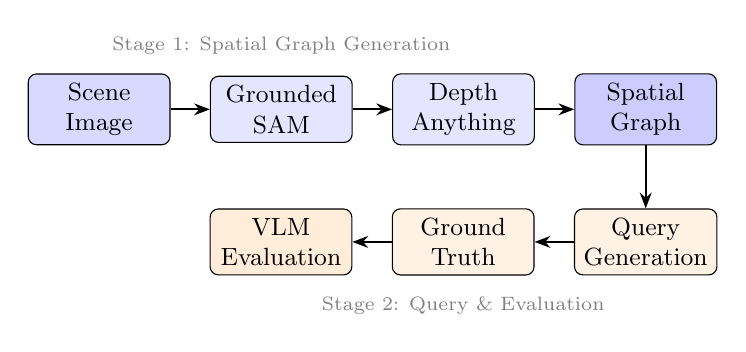
\begin{tikzpicture}[
    node distance=0.4cm,
    box/.style={rectangle, draw, rounded corners=3pt, minimum width=1.8cm, minimum height=0.6cm, align=center, font=\small},
    arrow/.style={-{Stealth[length=2mm]}, thick},
    label/.style={font=\scriptsize, color=gray}
]
% Stage 1: Spatial Graph Generation
\node[box, fill=blue!15] (img) {Scene\\Image};
\node[box, fill=blue!10, right=0.5cm of img] (det) {Grounded\\SAM};
\node[box, fill=blue!10, right=0.5cm of det] (depth) {Depth\\Anything};
\node[box, fill=blue!20, right=0.5cm of depth] (graph) {Spatial\\Graph};

% Stage 2: Query Generation & Evaluation
\node[box, fill=orange!10, below=0.8cm of graph] (query) {Query\\Generation};
\node[box, fill=orange!10, left=0.5cm of query] (gt) {Ground\\Truth};
\node[box, fill=orange!15, left=0.5cm of gt] (eval) {VLM\\Evaluation};

% Arrows
\draw[arrow] (img) -- (det);
\draw[arrow] (det) -- (depth);
\draw[arrow] (depth) -- (graph);
\draw[arrow] (graph) -- (query);
\draw[arrow] (query) -- (gt);
\draw[arrow] (gt) -- (eval);

% Stage labels
\node[label, above=0.15cm of det] {Stage 1: Spatial Graph Generation};
\node[label, below=0.15cm of gt] {Stage 2: Query \& Evaluation};

\end{tikzpicture}
\caption{Pipeline overview. Stage 1 constructs a spatial graph encoding object locations and relations. Stage 2 generates queries with geometric ground truth for exact-match evaluation.}
\label{fig:pipeline}
\end{figure}

\subsection{Spatial Graph Generation}

Given an input image, we construct a spatial graph $G = (V, E)$ where nodes $V$ represent detected objects and edges $E$ encode pairwise spatial relations. Each node stores object metadata (label, bounding box, segmentation mask, depth), and each edge stores the spatial relation between the connected objects.

\paragraph{Object detection and segmentation.} We employ Grounded-SAM, combining Grounding DINO for open-vocabulary detection with SAM for precise mask generation. Given a set of object category prompts, the model returns bounding boxes and segmentation masks for all detected instances. Each object receives a unique identifier by appending an instance index to its category label (e.g., \texttt{chair\_0}, \texttt{chair\_1}). We filter detections by confidence threshold and remove heavily overlapping boxes via non-maximum suppression.

\paragraph{Depth estimation.} We apply Depth Anything V2 to obtain a dense relative depth map $D \in \mathbb{R}^{H \times W}$, where lower values indicate closer proximity to the camera. For each detected object with segmentation mask $M_i$, we compute its representative depth as the median depth value within the mask: $d_i = \text{median}(\{D[p] : p \in M_i\})$. The median provides robustness to depth discontinuities at object boundaries.

\paragraph{Spatial relation computation.} For each ordered pair of objects $(o_i, o_j)$, we compute spatial relations along four axes by comparing their bounding box centers $(c_x, c_y)$ and depth values $d$:

\begin{itemize}[leftmargin=1.5em, itemsep=2pt, topsep=3pt]
    \item \textbf{Horizontal:} $o_i$ is \textit{left} of $o_j$ if $c_x^{(i)} < c_x^{(j)}$, else \textit{right}.
    \item \textbf{Vertical:} $o_i$ is \textit{above} $o_j$ if $c_y^{(i)} < c_y^{(j)}$, else \textit{below}.
    \item \textbf{Depth:} $o_i$ is \textit{in front of} $o_j$ if $d_i < d_j$ (closer to camera), else \textit{behind}.
    \item \textbf{Saliency:} $o_i$ is \textit{foreground} relative to $o_j$ if it is both closer (lower depth) and occupies a larger screen area, else \textit{background}.
\end{itemize}

Relations are stored as directed edges in the spatial graph, enabling efficient lookup during query generation.

\subsection{Query Taxonomy}

We organize queries along three orthogonal dimensions that isolate specific reasoning competencies.

\paragraph{Egocentric vs.\ Allocentric.} \textit{Egocentric} queries use the viewer's (camera's) reference frame: ``Is the chair to the left or right of the table?'' \textit{Allocentric} queries require perspective transformation by specifying an anchor object and facing direction: ``Standing at the chair facing the window, is the lamp to your left or right?'' This dimension tests mental rotation and reference frame transformation---a capability known to be challenging for both humans and models.

\paragraph{Viewer-centered vs.\ Object-to-object.} \textit{Viewer-centered} queries ask about object positions relative to the observer (``Which object is in the foreground?''), while \textit{object-to-object} queries ask about relations between two specific objects (``Is object A above or below object B?'').

\paragraph{Response format.} We include two formats: \textit{binary choice} (select between two relation labels, e.g., left vs.\ right) and \textit{multiple choice} (select among several labels, e.g., left/right/front/behind).

\subsection{Ground Truth Computation}

Ground truth answers are computed geometrically from the spatial graph, ensuring objective and reproducible evaluation without human annotation.

\paragraph{Egocentric relations.} Relations are computed directly in image coordinates. For a query about objects $o_i$ and $o_j$, we retrieve the precomputed relation from the spatial graph edge $(o_i, o_j)$.

\paragraph{Allocentric relations.} We transform the coordinate system to the anchor object's reference frame. Given anchor object $A$ at position $\mathbf{p}_A$ and facing direction toward object $F$ at $\mathbf{p}_F$, we define a local coordinate system with forward vector $\hat{\mathbf{f}} = (\mathbf{p}_F - \mathbf{p}_A) / \|\mathbf{p}_F - \mathbf{p}_A\|$. For a target object $T$, we compute its position relative to the anchor: $\mathbf{r} = \mathbf{p}_T - \mathbf{p}_A$. Left/right is determined by the sign of $\hat{\mathbf{f}} \times \mathbf{r}$ (cross product), and front/behind by the sign of $\hat{\mathbf{f}} \cdot \mathbf{r}$ (dot product).

\subsection{Evaluation Protocol}

\paragraph{Input format.} Models receive the scene image with overlaid bounding boxes and text labels, plus a natural language query. The visual annotation ensures models can identify referenced objects without requiring object detection capabilities, isolating spatial reasoning from perception.

\paragraph{Metrics.} We report accuracy as the fraction of correctly answered queries, with breakdowns by task type (egocentric/allocentric), frame type (viewer-centered/object-to-object), and relation axis (horizontal/vertical/depth) for fine-grained diagnosis of model capabilities.

%
% REQUIRED PACKAGES - Add to your main.tex preamble:
%   \usepackage{tikz}
%   \usetikzlibrary{positioning, arrows.meta, shapes.geometric, fit, backgrounds}
%
%=============================================================================

\section{Methodology}
\label{sec:methodology}

We present a benchmark for evaluating spatial reasoning in vision-language models that isolates relational reasoning from perceptual confounds. By providing labeled scene visualizations and structured queries with geometrically-computed ground truth, we enable precise diagnosis of model capabilities across spatial reasoning dimensions. Figure~\ref{fig:pipeline} illustrates our two-stage pipeline.

\begin{figure}[t]
\centering
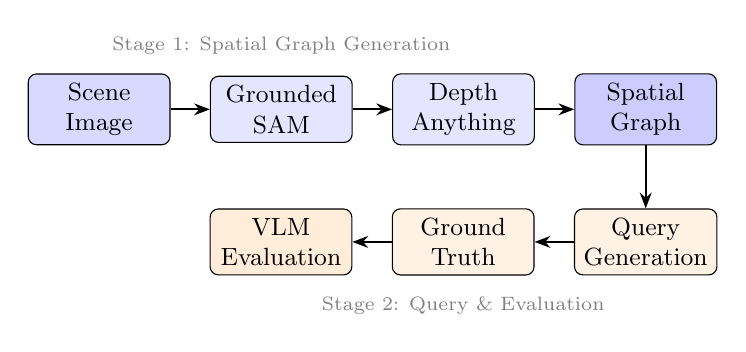
\begin{tikzpicture}[
    node distance=0.4cm,
    box/.style={rectangle, draw, rounded corners=3pt, minimum width=1.8cm, minimum height=0.6cm, align=center, font=\small},
    arrow/.style={-{Stealth[length=2mm]}, thick},
    label/.style={font=\scriptsize, color=gray}
]
% Stage 1: Spatial Graph Generation
\node[box, fill=blue!15] (img) {Scene\\Image};
\node[box, fill=blue!10, right=0.5cm of img] (det) {Grounded\\SAM};
\node[box, fill=blue!10, right=0.5cm of det] (depth) {Depth\\Anything};
\node[box, fill=blue!20, right=0.5cm of depth] (graph) {Spatial\\Graph};

% Stage 2: Query Generation & Evaluation
\node[box, fill=orange!10, below=0.8cm of graph] (query) {Query\\Generation};
\node[box, fill=orange!10, left=0.5cm of query] (gt) {Ground\\Truth};
\node[box, fill=orange!15, left=0.5cm of gt] (eval) {VLM\\Evaluation};

% Arrows
\draw[arrow] (img) -- (det);
\draw[arrow] (det) -- (depth);
\draw[arrow] (depth) -- (graph);
\draw[arrow] (graph) -- (query);
\draw[arrow] (query) -- (gt);
\draw[arrow] (gt) -- (eval);

% Stage labels
\node[label, above=0.15cm of det] {Stage 1: Spatial Graph Generation};
\node[label, below=0.15cm of gt] {Stage 2: Query \& Evaluation};

\end{tikzpicture}
\caption{Pipeline overview. Stage 1 constructs a spatial graph encoding object locations and relations. Stage 2 generates queries with geometric ground truth for exact-match evaluation.}
\label{fig:pipeline}
\end{figure}

\subsection{Spatial Graph Generation}

Given an input image, we construct a spatial graph $G = (V, E)$ where nodes $V$ represent detected objects and edges $E$ encode pairwise spatial relations. Each node stores object metadata (label, bounding box, segmentation mask, depth), and each edge stores the spatial relation between the connected objects.

\paragraph{Object detection and segmentation.} We employ Grounded-SAM, combining Grounding DINO for open-vocabulary detection with SAM for precise mask generation. Given a set of object category prompts, the model returns bounding boxes and segmentation masks for all detected instances. Each object receives a unique identifier by appending an instance index to its category label (e.g., \texttt{chair\_0}, \texttt{chair\_1}). We filter detections by confidence threshold and remove heavily overlapping boxes via non-maximum suppression.

\paragraph{Depth estimation.} We apply Depth Anything V2 to obtain a dense relative depth map $D \in \mathbb{R}^{H \times W}$, where lower values indicate closer proximity to the camera. For each detected object with segmentation mask $M_i$, we compute its representative depth as the median depth value within the mask: $d_i = \text{median}(\{D[p] : p \in M_i\})$. The median provides robustness to depth discontinuities at object boundaries.

\paragraph{Spatial relation computation.} For each ordered pair of objects $(o_i, o_j)$, we compute spatial relations along four axes by comparing their bounding box centers $(c_x, c_y)$ and depth values $d$:

\begin{itemize}[leftmargin=1.5em, itemsep=2pt, topsep=3pt]
    \item \textbf{Horizontal:} $o_i$ is \textit{left} of $o_j$ if $c_x^{(i)} < c_x^{(j)}$, else \textit{right}.
    \item \textbf{Vertical:} $o_i$ is \textit{above} $o_j$ if $c_y^{(i)} < c_y^{(j)}$, else \textit{below}.
    \item \textbf{Depth:} $o_i$ is \textit{in front of} $o_j$ if $d_i < d_j$ (closer to camera), else \textit{behind}.
    \item \textbf{Saliency:} $o_i$ is \textit{foreground} relative to $o_j$ if it is both closer (lower depth) and occupies a larger screen area, else \textit{background}.
\end{itemize}

Relations are stored as directed edges in the spatial graph, enabling efficient lookup during query generation.

\subsection{Query Taxonomy}

We organize queries along three orthogonal dimensions that isolate specific reasoning competencies.

\paragraph{Egocentric vs.\ Allocentric.} \textit{Egocentric} queries use the viewer's (camera's) reference frame: ``Is the chair to the left or right of the table?'' \textit{Allocentric} queries require perspective transformation by specifying an anchor object and facing direction: ``Standing at the chair facing the window, is the lamp to your left or right?'' This dimension tests mental rotation and reference frame transformation---a capability known to be challenging for both humans and models.

\paragraph{Viewer-centered vs.\ Object-to-object.} \textit{Viewer-centered} queries ask about object positions relative to the observer (``Which object is in the foreground?''), while \textit{object-to-object} queries ask about relations between two specific objects (``Is object A above or below object B?'').

\paragraph{Response format.} We include two formats: \textit{binary choice} (select between two relation labels, e.g., left vs.\ right) and \textit{multiple choice} (select among several labels, e.g., left/right/front/behind).

\subsection{Ground Truth Computation}

Ground truth answers are computed geometrically from the spatial graph, ensuring objective and reproducible evaluation without human annotation.

\paragraph{Egocentric relations.} Relations are computed directly in image coordinates. For a query about objects $o_i$ and $o_j$, we retrieve the precomputed relation from the spatial graph edge $(o_i, o_j)$.

\paragraph{Allocentric relations.} We transform the coordinate system to the anchor object's reference frame. Given anchor object $A$ at position $\mathbf{p}_A$ and facing direction toward object $F$ at $\mathbf{p}_F$, we define a local coordinate system with forward vector $\hat{\mathbf{f}} = (\mathbf{p}_F - \mathbf{p}_A) / \|\mathbf{p}_F - \mathbf{p}_A\|$. For a target object $T$, we compute its position relative to the anchor: $\mathbf{r} = \mathbf{p}_T - \mathbf{p}_A$. Left/right is determined by the sign of $\hat{\mathbf{f}} \times \mathbf{r}$ (cross product), and front/behind by the sign of $\hat{\mathbf{f}} \cdot \mathbf{r}$ (dot product).

\subsection{Evaluation Protocol}

\paragraph{Input format.} Models receive the scene image with overlaid bounding boxes and text labels, plus a natural language query. The visual annotation ensures models can identify referenced objects without requiring object detection capabilities, isolating spatial reasoning from perception.

\paragraph{Metrics.} We report accuracy as the fraction of correctly answered queries, with breakdowns by task type (egocentric/allocentric), frame type (viewer-centered/object-to-object), and relation axis (horizontal/vertical/depth) for fine-grained diagnosis of model capabilities.


%-----------------------------------------------------------------------------
% RESULTS
%-----------------------------------------------------------------------------
\section{Results}
\label{sec:results}

%=============================================================================
% BENCHMARK RESULTS SECTION - Condensed (2 pages, 2 tables)
%=============================================================================

We evaluate three vision-language models on our spatial reasoning benchmark: GPT-5-mini (OpenAI), Claude Haiku 4.5 (Anthropic), and Qwen2.5-VL-7B (Alibaba). Each model receives the annotated scene image and a structured query, responding with a spatial relation label. The evaluation spans 50 images with 3,672 total queries.

\subsection{Overall Performance}

Table~\ref{tab:overall_results} presents overall accuracy by task type. All three models achieve above-chance performance, but substantial gaps exist between egocentric and allocentric reasoning tasks.

\begin{table}[h]
\centering
\caption{Overall spatial reasoning accuracy by task type. GPT-5-mini shows the largest egocentric-allocentric gap despite achieving the best egocentric performance.}
\label{tab:overall_results}
\begin{tabular}{@{}lccc|c@{}}
\toprule
\textbf{Model} & \textbf{Egocentric} & \textbf{Allocentric} & \textbf{Gap} & \textbf{Overall} \\
\midrule
Qwen2.5-VL-7B & 63.9\% & 52.8\% & 11.1 & \textbf{59.8\%} \\
GPT-5-mini & \textbf{66.7\%} & 39.9\% & \textbf{26.8} & 56.8\% \\
Claude Haiku 4.5 & 57.4\% & 47.6\% & 9.8 & 53.8\% \\
\bottomrule
\end{tabular}
\end{table}

Qwen2.5-VL-7B achieves the highest overall accuracy (59.8\%), followed by GPT-5-mini (56.8\%) and Claude Haiku 4.5 (53.8\%). Notably, GPT-5-mini---a reasoning model that employs internal chain-of-thought---achieves the best egocentric accuracy (66.7\%) but exhibits the largest egocentric-allocentric gap (26.8 percentage points), more than double that of the other models. This suggests that while reasoning capabilities enhance straightforward spatial judgments, they may not transfer effectively to perspective transformation tasks.

All models show relatively balanced performance between viewer-centered and object-to-object frame types (differences $<$3 percentage points), indicating that frame type alone does not significantly affect performance. However, substantial variation exists across relation axes: vertical relations (above/below) achieve the highest accuracy across all models (65--71\%), while left/right relations prove most challenging for GPT-5-mini (47.6\% overall, driven by allocentric failures).

\subsection{Hierarchical Breakdown}

Table~\ref{tab:hierarchical} provides a fine-grained breakdown by task type, frame type, and relation axis. This hierarchical view reveals specific failure patterns obscured by aggregate metrics.

\begin{table}[h]
\centering
\small
\caption{Hierarchical accuracy breakdown (\%). \colorbox{red!15}{Red} indicates accuracy below 40\% (critical failure), \colorbox{yellow!25}{yellow} indicates 40--50\% (below chance for binary).}
\label{tab:hierarchical}
\setlength{\tabcolsep}{3.5pt}
\begin{tabular}{@{}ll|ccc@{}}
\toprule
\textbf{Task / Frame} & \textbf{Relation} & \textbf{GPT-5-mini} & \textbf{Claude} & \textbf{Qwen} \\
\midrule
\multirow{3}{*}{Ego / Viewer}
    & above/below & 68.9 & 62.9 & 65.4 \\
    & fg/bg & 60.1 & 55.3 & 60.4 \\
    & left/right & 63.6 & 58.7 & 61.2 \\
\midrule
\multirow{3}{*}{Ego / Obj-Obj}
    & above/below & 72.4 & 64.1 & 65.4 \\
    & front/behind & 69.9 & 52.0 & 53.6 \\
    & left/right & 65.3 & 51.5 & 61.2 \\
\midrule
\multirow{2}{*}{Allo / Viewer}
    & front/behind & 58.2 & \cellcolor{yellow!25}49.0 & 52.8 \\
    & left/right & \cellcolor{red!15}32.9 & 50.0 & 52.8 \\
\midrule
\multirow{2}{*}{Allo / Obj-Obj}
    & front/behind & \cellcolor{yellow!25}41.3 & \cellcolor{yellow!25}41.7 & 52.8 \\
    & left/right & \cellcolor{red!15}23.3 & \cellcolor{yellow!25}48.6 & 52.8 \\
\bottomrule
\end{tabular}
\end{table}

The hierarchical breakdown reveals distinct failure patterns across models. GPT-5-mini exhibits a critical failure mode on allocentric left/right queries: object-to-object accuracy drops to 23.3\% and viewer-centered to 32.9\%---well below the 50\% chance level for binary choices. This indicates that despite strong reasoning capabilities for egocentric tasks (65--72\% on egocentric left/right), GPT-5-mini systematically fails at lateral perspective transformation. The model appears to confuse left and right when reasoning from another object's viewpoint.

Claude Haiku 4.5 and Qwen2.5-VL-7B show more balanced performance across conditions. Claude achieves moderate accuracy uniformly but struggles with allocentric front/behind relations (41.7\% object-to-object). Qwen maintains the most consistent performance, never dropping below 52\% on any condition, suggesting more robust (though not superior) spatial representations.

\subsection{Summary of Findings}

Our benchmark evaluation reveals three key patterns. First, reasoning models show amplified egocentric-allocentric gaps: GPT-5-mini achieves the best egocentric performance but the worst allocentric performance, resulting in a 26.8 percentage point gap. This suggests that chain-of-thought reasoning may not transfer to---or may even impede---perspective transformation tasks.

Second, left/right allocentric transformations are particularly challenging. This category shows the largest failures, with GPT-5-mini dropping to near-random performance (23--33\%). Mental rotation for lateral directions poses a specific computational challenge that current VLMs struggle to solve.

Third, different models exhibit distinct weaknesses: GPT-5-mini excels at egocentric tasks but fails catastrophically on allocentric left/right; Claude Haiku 4.5 shows uniform but moderate performance; Qwen2.5-VL-7B achieves the best balance across conditions. These patterns suggest that architecture and training approach, rather than scale alone, determine spatial reasoning capabilities.


%-----------------------------------------------------------------------------
% MECHANISTIC ANALYSIS
%-----------------------------------------------------------------------------
%=============================================================================
% SPATIAL ANALYSIS SECTION
% For inclusion in main NeurIPS 2025 document
%=============================================================================
%
% USAGE: Add %=============================================================================
% SPATIAL ANALYSIS SECTION
% For inclusion in main NeurIPS 2025 document
%=============================================================================
%
% USAGE: Add %=============================================================================
% SPATIAL ANALYSIS SECTION
% For inclusion in main NeurIPS 2025 document
%=============================================================================
%
% USAGE: Add \input{spatial_analysis_section} in your Results section
%
% REQUIRED PACKAGES - Add these to your main.tex preamble:
%   \usepackage{siunitx}
%
% REQUIRED FILES:
%   figures/mechanistic_analysis.pdf (or .png)
%
% Note: booktabs, multirow, graphicx are already in your main.tex
%=============================================================================

\subsection{Mechanistic Analysis of Spatial Reasoning}
\label{sec:mechanistic}

Beyond aggregate accuracy metrics, we seek to understand \textit{why} models succeed or fail at spatial reasoning. To this end, we conduct mechanistic analysis on Qwen2.5-VL-7B (8.29B parameters), extracting internal activations and attention patterns to identify neural correlates of correct spatial reasoning.

\paragraph{Method.}

We evaluate Qwen2.5-VL-7B on 50 COCO images, generating \num{3672} spatial queries that span all task types, frame types, and relation axes defined in our benchmark. Table~\ref{tab:qwen_eval} summarizes the results: the model achieves 63.9\% accuracy on egocentric tasks but only 52.8\% on allocentric tasks, confirming an 11.1 percentage point gap that indicates perspective transformation poses substantial difficulty.

\begin{table}[h]
\centering
\small
\caption{Qwen2.5-VL-7B spatial reasoning accuracy on \num{3672} queries across 50 COCO images.}
\label{tab:qwen_eval}
\begin{tabular}{@{}lcc@{}}
\toprule
\textbf{Task Type} & \textbf{Accuracy (\%)} & \textbf{Correct / Total} \\
\midrule
Egocentric  & 63.9 & 1477 / 2312 \\
Allocentric & 52.8 & 718 / 1360 \\
\midrule
\textbf{Overall} & \textbf{59.8} & \textbf{2195 / 3672} \\
\bottomrule
\end{tabular}
\end{table}

To probe the internal mechanisms underlying these accuracy differences, we sample 33 cases---17 correct and 16 incorrect predictions---and extract two complementary signals. First, we compute \textit{activation norms} (L2 norm of hidden states) at each layer, measuring representation strength. Second, we compute the \textit{image attention ratio}, defined as the fraction of attention weights directed to image tokens versus text tokens, quantifying how strongly the model grounds its reasoning in visual content.

\paragraph{Results.}

Figure~\ref{fig:mechanistic} presents our findings across three panels. Panel~(A) shows activation norms across the model's layers, from early vision blocks through the language model. Notably, success and failure cases exhibit nearly identical activation patterns throughout the network, indicating that raw representation magnitude does not differentiate correct from incorrect predictions. This null result is informative: it suggests that failures do not stem from weak or degraded representations, but rather from how those representations are used.

\begin{figure}[t]
\centering
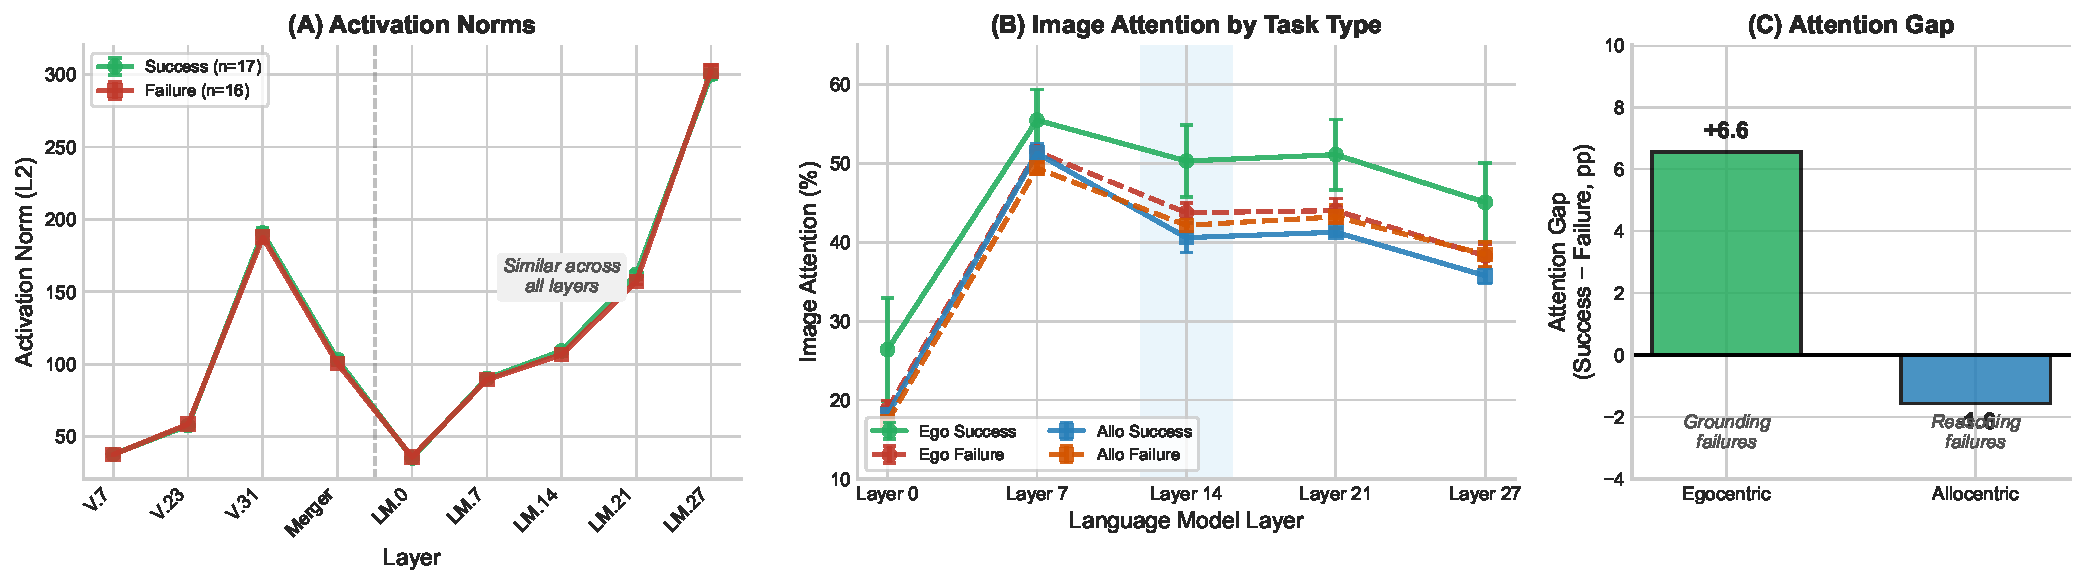
\includegraphics[width=\linewidth]{figures/mechanistic_analysis.pdf}
\caption{\textbf{Mechanistic analysis of spatial reasoning.} (A)~Activation norms show no difference between success and failure cases across all layers, indicating that representation strength alone does not predict correctness. (B)~Image attention ratio reveals task-specific patterns: egocentric success cases (green solid) consistently attend more to image tokens than failures (red dashed), while allocentric cases show no such separation. (C)~At Layer~14, egocentric tasks exhibit a +6.6 percentage point attention advantage for successful predictions (grounding failures), whereas allocentric tasks show --1.6 percentage points (reasoning failures).}
\label{fig:mechanistic}
\end{figure}

The key differentiation emerges in attention patterns, shown in Panel~(B). For egocentric tasks, a clear separation appears: successful predictions (green solid line) consistently maintain higher image attention than failures (red dashed line) across all language model layers, with the gap most pronounced at Layer~14. In contrast, allocentric tasks show no such separation---the success and failure lines interleave throughout the network, with successful predictions sometimes showing \textit{lower} image attention than failures.

Panel~(C) quantifies this divergence at Layer~14. For egocentric tasks, successful predictions exhibit 6.6 percentage points higher image attention than failures (50.3\% vs.\ 43.8\%). This pattern indicates that egocentric failures are fundamentally \textit{grounding failures}---the model does not sufficiently attend to visual content when it answers incorrectly. For allocentric tasks, successful predictions show 1.6 percentage points \textit{lower} attention to image tokens than failures (40.6\% vs.\ 42.2\%). This reversal indicates that allocentric failures are \textit{reasoning failures}: the model attends to the image adequately but cannot correctly perform the perspective transformation required to answer from an object's viewpoint.

\paragraph{Takeaways.}

These findings reveal that spatial reasoning failures arise from fundamentally different mechanisms depending on task type. The similarity in activation norms rules out representation degradation as a failure mode; instead, the divergence appears in how attention is allocated. For egocentric reasoning, success correlates with stronger visual grounding, suggesting that attention-focused training or architectural modifications could yield improvements. For allocentric reasoning, however, the absence of an attention deficit points to a deeper limitation in perspective-taking capabilities, which may require explicit modules or training objectives that teach reference frame transformation.
 in your Results section
%
% REQUIRED PACKAGES - Add these to your main.tex preamble:
%   \usepackage{siunitx}
%
% REQUIRED FILES:
%   figures/mechanistic_analysis.pdf (or .png)
%
% Note: booktabs, multirow, graphicx are already in your main.tex
%=============================================================================

\subsection{Mechanistic Analysis of Spatial Reasoning}
\label{sec:mechanistic}

Beyond aggregate accuracy metrics, we seek to understand \textit{why} models succeed or fail at spatial reasoning. To this end, we conduct mechanistic analysis on Qwen2.5-VL-7B (8.29B parameters), extracting internal activations and attention patterns to identify neural correlates of correct spatial reasoning.

\paragraph{Method.}

We evaluate Qwen2.5-VL-7B on 50 COCO images, generating \num{3672} spatial queries that span all task types, frame types, and relation axes defined in our benchmark. Table~\ref{tab:qwen_eval} summarizes the results: the model achieves 63.9\% accuracy on egocentric tasks but only 52.8\% on allocentric tasks, confirming an 11.1 percentage point gap that indicates perspective transformation poses substantial difficulty.

\begin{table}[h]
\centering
\small
\caption{Qwen2.5-VL-7B spatial reasoning accuracy on \num{3672} queries across 50 COCO images.}
\label{tab:qwen_eval}
\begin{tabular}{@{}lcc@{}}
\toprule
\textbf{Task Type} & \textbf{Accuracy (\%)} & \textbf{Correct / Total} \\
\midrule
Egocentric  & 63.9 & 1477 / 2312 \\
Allocentric & 52.8 & 718 / 1360 \\
\midrule
\textbf{Overall} & \textbf{59.8} & \textbf{2195 / 3672} \\
\bottomrule
\end{tabular}
\end{table}

To probe the internal mechanisms underlying these accuracy differences, we sample 33 cases---17 correct and 16 incorrect predictions---and extract two complementary signals. First, we compute \textit{activation norms} (L2 norm of hidden states) at each layer, measuring representation strength. Second, we compute the \textit{image attention ratio}, defined as the fraction of attention weights directed to image tokens versus text tokens, quantifying how strongly the model grounds its reasoning in visual content.

\paragraph{Results.}

Figure~\ref{fig:mechanistic} presents our findings across three panels. Panel~(A) shows activation norms across the model's layers, from early vision blocks through the language model. Notably, success and failure cases exhibit nearly identical activation patterns throughout the network, indicating that raw representation magnitude does not differentiate correct from incorrect predictions. This null result is informative: it suggests that failures do not stem from weak or degraded representations, but rather from how those representations are used.

\begin{figure}[t]
\centering
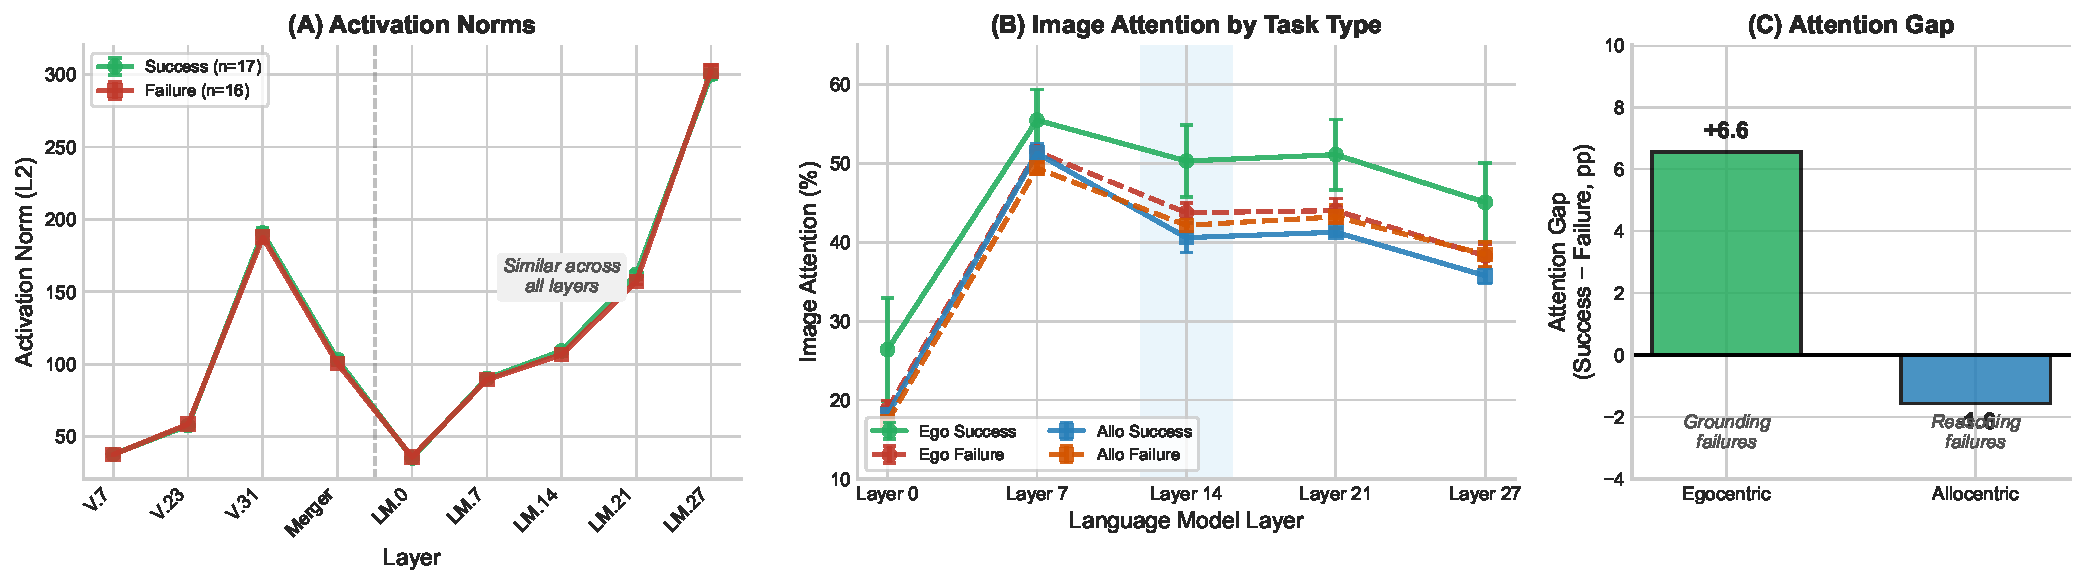
\includegraphics[width=\linewidth]{figures/mechanistic_analysis.pdf}
\caption{\textbf{Mechanistic analysis of spatial reasoning.} (A)~Activation norms show no difference between success and failure cases across all layers, indicating that representation strength alone does not predict correctness. (B)~Image attention ratio reveals task-specific patterns: egocentric success cases (green solid) consistently attend more to image tokens than failures (red dashed), while allocentric cases show no such separation. (C)~At Layer~14, egocentric tasks exhibit a +6.6 percentage point attention advantage for successful predictions (grounding failures), whereas allocentric tasks show --1.6 percentage points (reasoning failures).}
\label{fig:mechanistic}
\end{figure}

The key differentiation emerges in attention patterns, shown in Panel~(B). For egocentric tasks, a clear separation appears: successful predictions (green solid line) consistently maintain higher image attention than failures (red dashed line) across all language model layers, with the gap most pronounced at Layer~14. In contrast, allocentric tasks show no such separation---the success and failure lines interleave throughout the network, with successful predictions sometimes showing \textit{lower} image attention than failures.

Panel~(C) quantifies this divergence at Layer~14. For egocentric tasks, successful predictions exhibit 6.6 percentage points higher image attention than failures (50.3\% vs.\ 43.8\%). This pattern indicates that egocentric failures are fundamentally \textit{grounding failures}---the model does not sufficiently attend to visual content when it answers incorrectly. For allocentric tasks, successful predictions show 1.6 percentage points \textit{lower} attention to image tokens than failures (40.6\% vs.\ 42.2\%). This reversal indicates that allocentric failures are \textit{reasoning failures}: the model attends to the image adequately but cannot correctly perform the perspective transformation required to answer from an object's viewpoint.

\paragraph{Takeaways.}

These findings reveal that spatial reasoning failures arise from fundamentally different mechanisms depending on task type. The similarity in activation norms rules out representation degradation as a failure mode; instead, the divergence appears in how attention is allocated. For egocentric reasoning, success correlates with stronger visual grounding, suggesting that attention-focused training or architectural modifications could yield improvements. For allocentric reasoning, however, the absence of an attention deficit points to a deeper limitation in perspective-taking capabilities, which may require explicit modules or training objectives that teach reference frame transformation.
 in your Results section
%
% REQUIRED PACKAGES - Add these to your main.tex preamble:
%   \usepackage{siunitx}
%
% REQUIRED FILES:
%   figures/mechanistic_analysis.pdf (or .png)
%
% Note: booktabs, multirow, graphicx are already in your main.tex
%=============================================================================

\subsection{Mechanistic Analysis of Spatial Reasoning}
\label{sec:mechanistic}

Beyond aggregate accuracy metrics, we seek to understand \textit{why} models succeed or fail at spatial reasoning. To this end, we conduct mechanistic analysis on Qwen2.5-VL-7B (8.29B parameters), extracting internal activations and attention patterns to identify neural correlates of correct spatial reasoning.

\paragraph{Method.}

We evaluate Qwen2.5-VL-7B on 50 COCO images, generating \num{3672} spatial queries that span all task types, frame types, and relation axes defined in our benchmark. Table~\ref{tab:qwen_eval} summarizes the results: the model achieves 63.9\% accuracy on egocentric tasks but only 52.8\% on allocentric tasks, confirming an 11.1 percentage point gap that indicates perspective transformation poses substantial difficulty.

\begin{table}[h]
\centering
\small
\caption{Qwen2.5-VL-7B spatial reasoning accuracy on \num{3672} queries across 50 COCO images.}
\label{tab:qwen_eval}
\begin{tabular}{@{}lcc@{}}
\toprule
\textbf{Task Type} & \textbf{Accuracy (\%)} & \textbf{Correct / Total} \\
\midrule
Egocentric  & 63.9 & 1477 / 2312 \\
Allocentric & 52.8 & 718 / 1360 \\
\midrule
\textbf{Overall} & \textbf{59.8} & \textbf{2195 / 3672} \\
\bottomrule
\end{tabular}
\end{table}

To probe the internal mechanisms underlying these accuracy differences, we sample 33 cases---17 correct and 16 incorrect predictions---and extract two complementary signals. First, we compute \textit{activation norms} (L2 norm of hidden states) at each layer, measuring representation strength. Second, we compute the \textit{image attention ratio}, defined as the fraction of attention weights directed to image tokens versus text tokens, quantifying how strongly the model grounds its reasoning in visual content.

\paragraph{Results.}

Figure~\ref{fig:mechanistic} presents our findings across three panels. Panel~(A) shows activation norms across the model's layers, from early vision blocks through the language model. Notably, success and failure cases exhibit nearly identical activation patterns throughout the network, indicating that raw representation magnitude does not differentiate correct from incorrect predictions. This null result is informative: it suggests that failures do not stem from weak or degraded representations, but rather from how those representations are used.

\begin{figure}[t]
\centering
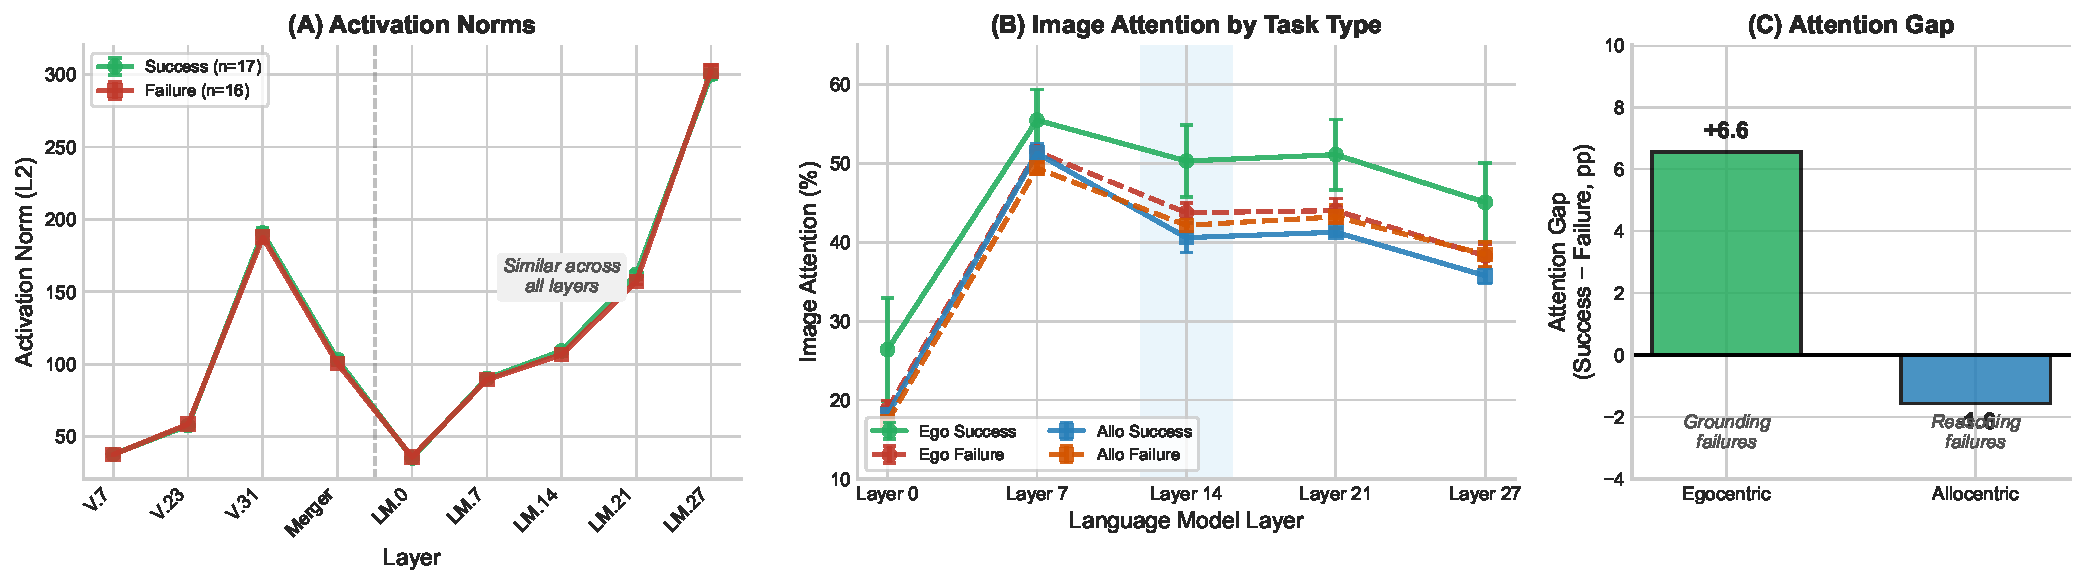
\includegraphics[width=\linewidth]{figures/mechanistic_analysis.pdf}
\caption{\textbf{Mechanistic analysis of spatial reasoning.} (A)~Activation norms show no difference between success and failure cases across all layers, indicating that representation strength alone does not predict correctness. (B)~Image attention ratio reveals task-specific patterns: egocentric success cases (green solid) consistently attend more to image tokens than failures (red dashed), while allocentric cases show no such separation. (C)~At Layer~14, egocentric tasks exhibit a +6.6 percentage point attention advantage for successful predictions (grounding failures), whereas allocentric tasks show --1.6 percentage points (reasoning failures).}
\label{fig:mechanistic}
\end{figure}

The key differentiation emerges in attention patterns, shown in Panel~(B). For egocentric tasks, a clear separation appears: successful predictions (green solid line) consistently maintain higher image attention than failures (red dashed line) across all language model layers, with the gap most pronounced at Layer~14. In contrast, allocentric tasks show no such separation---the success and failure lines interleave throughout the network, with successful predictions sometimes showing \textit{lower} image attention than failures.

Panel~(C) quantifies this divergence at Layer~14. For egocentric tasks, successful predictions exhibit 6.6 percentage points higher image attention than failures (50.3\% vs.\ 43.8\%). This pattern indicates that egocentric failures are fundamentally \textit{grounding failures}---the model does not sufficiently attend to visual content when it answers incorrectly. For allocentric tasks, successful predictions show 1.6 percentage points \textit{lower} attention to image tokens than failures (40.6\% vs.\ 42.2\%). This reversal indicates that allocentric failures are \textit{reasoning failures}: the model attends to the image adequately but cannot correctly perform the perspective transformation required to answer from an object's viewpoint.

\paragraph{Takeaways.}

These findings reveal that spatial reasoning failures arise from fundamentally different mechanisms depending on task type. The similarity in activation norms rules out representation degradation as a failure mode; instead, the divergence appears in how attention is allocated. For egocentric reasoning, success correlates with stronger visual grounding, suggesting that attention-focused training or architectural modifications could yield improvements. For allocentric reasoning, however, the absence of an attention deficit points to a deeper limitation in perspective-taking capabilities, which may require explicit modules or training objectives that teach reference frame transformation.


%-----------------------------------------------------------------------------
% CONCLUSION
%-----------------------------------------------------------------------------
\section{Conclusion}
\label{sec:conclusion}

% TODO: Write conclusion
% - Summary of contributions
% - Key findings: egocentric-allocentric gap, distinct failure mechanisms
% - Implications for VLM development
% - Future work: intervention studies, more models, embodied evaluation

%-----------------------------------------------------------------------------
% REFERENCES
%-----------------------------------------------------------------------------
\bibliographystyle{plainnat}
\bibliography{references}

\end{document}
